\chapter{Banco de Dados Geográfico}
\label{cap:bd}

\section{Introdução}

Os bancos de dados geográficos têm como principal característica suportar feições geométricas em suas tabelas, além de oferecer a possibilidade de análise e consultas espaciais. Em outras palavras, esse tipo de banco possibilita a realização de cálculos como áreas e distâncias além de realizar a geração de \textit{buffers} (zona de influência) e outras operações entre as geometrias.

Ao decorrer dos anos, os Sistemas de Informações Geográficos (SIGs) seguiram diferentes formas de implementação, principalmente em relação a estratégia utilizada para armazenar e recuperar dados espaciais. Mais recentemente, os SIGs passaram a utilizar cada vez mais os recursos dos Sistemas Gerenciadores de Banco de Dados (SGBDs), principalmente com o surgimento de extensões espaciais, o que facilitou o desenvolvimento do banco de dados geográfico dos SIGs \cite{gisasp}.

Nas seções deste capítulo, são abordados os principais conceitos relacionados ao paradigma dos quatro universos, modelagem conceitual de dados geográfico, modelo de dados OMT-G, sistema gerenciador de banco de dados, PostGIS e consultas espaciais.

\section{Paradigma dos Quatro Universos}
\label{quatro-universos}

Geoinformação é toda informação passível de espacialização, ou seja, que possua algum tipo de vínculo geográfico que permite sua localização. Este pode ser um ponto, um endereço, um território, entre outros. O problema da geoinformação é a representação computacional do espaço geográfico \cite{harley}.

Para realizar representações computacionais do espaço geográfico, é usado o conceito conhecido como “paradigma dos quatro universos” \cite{velhogomes}. Este paradigma é representado pelo universo ontológico, universo formal, universo estrutural e universo de implementação, como apresentado na Figura \ref{fig:QuatroUniversos}.

\begin{figure}[h]
\centering
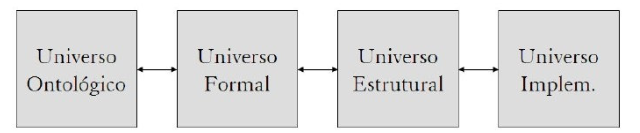
\includegraphics[width=0.65\textwidth]{./img/cap_II/1-QuatroUniversos}
\caption{Paradigma dos quatro universos \cite{queirozferreira}.}
\label{fig:QuatroUniversos}
\end{figure}

A partir do paradigma dos quatro universos, é possível resolver a complexidade que existe entre o mundo real e o mundo computacional.

\subsection{Universo Ontológico}

O universo ontológico inclui os conceitos da realidade a serem modelados no sistema computacional, como os tipos de solo, elementos de cadastro urbano ou rural, dados geofísicos e topográficos.

Um sistema de informação pode ser concebido como um mecanismo de comunicação entre duas partes: o produtor e o usuário. Para que funcione, é necessário que haja uma concordância entre os conceitos das partes. Numa perspectiva mais geral, seu sucesso depende da existência de uma comunidade que compartilhe as definições utilizadas para construí-lo. Para construir um sistema de informação, é preciso definir qual dos diferentes conceitos será representado, como esta representação será construída, e como o usuário pode compreender as características e limitações desta representação. Deste modo, o problema fundamental de um sistema de informação é definir o conjunto de conceitos a ser representado \cite{queirozferreira}.

Para os dados geográficos, uma geo-ontologia é um conjunto de conceitos e um conjunto de relações semânticas e espaciais entre estes termos. Cada conceito tem um nome, uma definição e um conjunto de atributos. O conjunto das relações semânticas inclui as relações de sinonímia, similaridade, e especialização. Os Sistemas de Informações Geográficos (SIGs) e dados geográficos possuem ontologias descritas através do formato \textit{Geographic Markup Language} (GML), proposto pelo consórcio \textit{Open Geospatial Consortium} (OGC) (que será abordado no Capítulo \ref{cap:sig}) \cite{queirozferreira}.

\subsection{Universo Formal}

O universo formal representa um componente intermediário entre os conceitos do universo ontológico e as estruturas de dados e algoritmos computacionais. No universo formal, buscamos estabelecer um conjunto de entidades lógicas que agrupem os diferentes conceitos da ontologia de aplicação da forma mais abrangente possível. O universo formal se divide em duas partes: como medir o mundo real e como generalizar os conceitos da ontologia em entidades formais abrangentes \cite{queirozferreira}.

\subsubsection{Atributos de Dados Geográficos: Teoria da Medida}

Para representar dados geográficos no computador, temos de descrever sua variação no espaço e no tempo. O processo de medida consiste em associar números ou símbolos a diferentes ocorrências de um mesmo atributo, para que a relação dos números ou símbolos reflita as relações entre as ocorrências mensuradas. Por exemplo, podemos medir a poluição do ar em uma cidade em diferentes locais, e cada um desses locais dará um resultado diferente. Esta atribuição é denominada escala de medida \cite{queirozferreira}. Stevens \citeonline{stevens} afirma que há quatro escalas de mensuração: nominal, ordinal, intervalo e razão.

\begin{itemize}
\item A escala nominal classifica objetos em classes distintas sem ordem inerente, como rótulos que podem ser quaisquer símbolos. A Figura \ref{fig:TeoriaMedida} representa a escala nominal.
\item A escala ordinal introduz a idéia de ordenação, caracterizando os objetos em classes distintas que possuem uma ordem natural (por exemplo 1 – ruim, 2 – bom, 3 – ótimo ou “0-10\%”, “11-20\%”, “mais que 20\%”). A Figura \ref{fig:TeoriaMedida} representa a escala ordinal;
\item A escala por intervalo possui um ponto zero arbitrário, uma distância proporcional entre os intervalos e uma faixa de medidas entre [-infinito, +infinito]. A temperatura em graus \textit{Celsius} é um exemplo de medida por intervalo, onde o ponto zero corresponde a uma convenção (a fusão do gelo em água);
\item A escala de razão permite um tratamento mais analítico da informação, pois nela o ponto de referência zero não é arbitrário, mas determinado por alguma condição natural. Sua faixa de valores é limitada entre [0, infinito]. Nesta escala existe um ponto zero absoluto que não pode ser alterado e um intervalo arbitrário com distâncias proporcionais entre os intervalos.
\end{itemize}

\newpage

\begin{figure}[h]
\centering
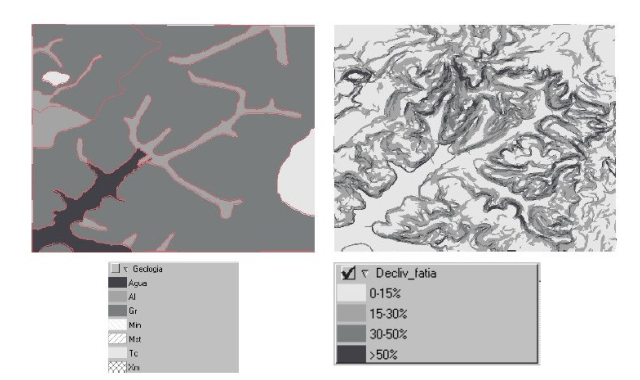
\includegraphics[width=0.75\textwidth]{./img/cap_II/2-TeoriaMedida}
\caption{Exemplo de medida nominal (mapa geológico a esquerda) e medida ordinal (mapa de classes de declividade a direita) \cite{queirozferreira}.}
\label{fig:TeoriaMedida}
\end{figure}

A Tabela \ref{tabela-medidas-geograficas} apresenta um resumo das escalas de medidas, destaca a característica principal, apresenta algumas operações admitidas e exemplos para cada uma delas \cite{queirozferreira}.

\begin{table}[htb]
\IBGEtab{
\caption{Tipo de medidas de dados geográficos \cite{queirozferreira}.}
\label{tabela-medidas-geograficas}
}{
\begin{tabular}{llll}
\toprule
Escala & Características & Exemplos & Operações Possíveis\\
\midrule \midrule
Nominal & Descrição & Tipo de solo, vegetação, uso do solo & Seleção, comparação\\
\midrule
Ordinal & Ordem & Classes de declividade, aptidão de uso & Mediana, máximo, mínimo\\
\midrule
Intervalo & Distância & Altimetria & Diferença, soma\\
\midrule
Razão & Valores absolutos & Renda, população, taxa de natalidade & Operações aritméticas\\
\bottomrule
\end{tabular}}{}
\end{table}

\subsubsection{Espaço Absoluto e Espaço Relativo}

A representação no espaço absoluto se dá através das coordenadas das fronteiras, na Figura \ref{fig:AbsolutoRelativo}, é mostrado a esquerda os distritos da cidade de São Paulo identificados por suas fronteiras. Essa Figura representa o espaço absoluto, pois as fronteiras são estabelecidas na legislação brasileira. E já na imagem da direita, é mostrado um grafo com as conexões dos distritos que formam uma rede, ou seja, a localização exata de cada distrito não é armazenada, pois a rede só captura as relações de adjacência. Essa rede de conexão dos distritos é um modelo de espaço relativo \cite{queirozferreira}.

Para um projeto de um SIG, é fundamental a escolha do tipo de representação que será usado. Esta escolha depende basicamente do tipo de análise a ser realizada pelo sistema. Representações em espaço absoluto são usualmente utilizadas quando as consultas espaciais a serem realizadas envolvem entidades de tipos diferentes. Quando os procedimentos de análise envolvem apenas as relações de conectividade, como, quando se precisa saber o caminho mais curto entre dois distritos \cite{queirozferreira}. Por exemplo, quando se quer saber os municípios vizinhos de uma cidade.

\newpage

\begin{figure}[h]
\centering
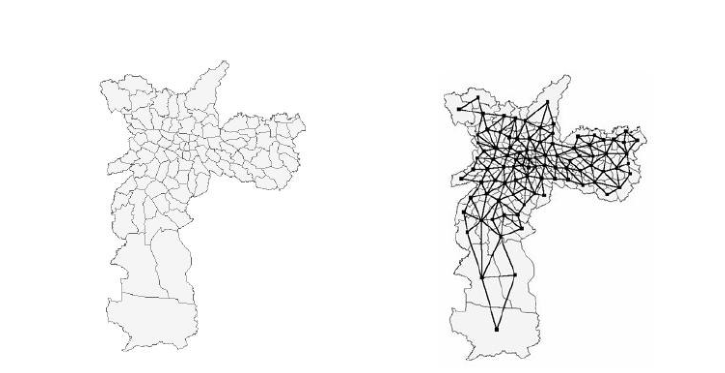
\includegraphics[width=0.75\textwidth]{./img/cap_II/3-AbsolutoRelativo}
\caption{Dualidade entre espaço absoluto e espaço relativo \cite{queirozferreira}.}
\label{fig:AbsolutoRelativo}
\end{figure}

\subsubsection{Modelos no Espaço Absoluto: Geo-Campos e Geo-Objetos}

Existem dois modelos formais para entidades geográficas no espaço absoluto: geo-campos e geo-objetos. O modelo de geo-campos enxerga o espaço geográfico como uma superfície contínua, sobre a qual variam os fenômenos a serem observados. Por exemplo, um mapa de vegetação associa a cada ponto do mapa um tipo específico de cobertura vegetal \cite{queirozferreira}.

O modelo de geo-objetos representa o espaço geográfico como uma coleção de entidades distintas e identificáveis, onde cada entidade é definida por uma fronteira fechada. Por exemplo, um cadastro urbano identifica cada lote como um dado individual, com atributos que o distinguem dos demais \cite{queirozferreira}.

A diferença essencial entre um geo-campo e um geo-objeto é o papel da fronteira, representada na Figura \ref{fig:Geo-CamposObjetos}. A fronteira de um geo-campo é uma divisão arbitrária relacionada apenas com nossa capacidade de medida. Assim, o geo-campo pode ser dividido em partes e ainda assim manter sua propriedade essencial (que é sua função de atributo). Por contraste, um geo-objeto é essencialmente definido por sua fronteira, que o separa do mundo exterior. Ele não pode ser dividido e mantem suas propriedades essenciais. Dentro da fronteira, todas as propriedades do objeto são constantes \cite{queirozferreira}.

\begin{figure}[h]
\centering
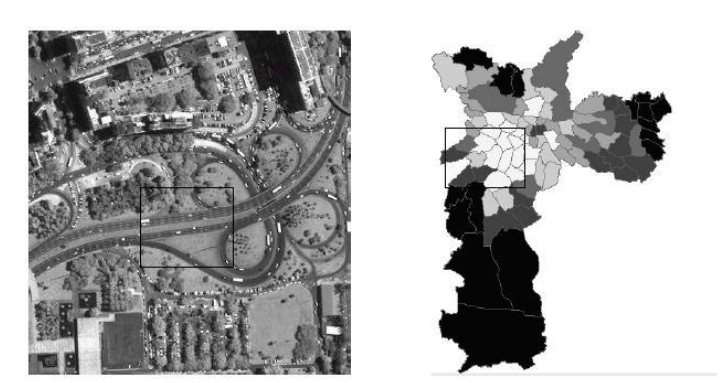
\includegraphics[width=0.75\textwidth]{./img/cap_II/4-Geo-CamposObjetos}
\caption{Exemplo de geo-campo e de geo-objetos \cite{queirozferreira}.}
\label{fig:Geo-CamposObjetos}
\end{figure}

\newpage

\subsubsection{Modelos no Espaço Relativo: Redes}

O modelo de redes concebe o espaço geográfico como um conjunto de pontos no espaço (chamados de nós), conectados por linhas (chamados arcos), onde tanto os nós quanto os arcos possuem atributos. A topologia de redes constitui um grafo onde os recursos que fluem localização geográficas distintas são gravadas \cite{queirozferreira}.

Os fenômenos modelados por redes estão relacionados ao fluxo de pessoas ou materiais, a conexões de influência, a linhas de comunicação e acessibilidade, como por exemplo, na representação dos serviços de utilidade pública, como água, luz e telefone, na representação de rodovias e redes de drenagem (bacias hidrográficas) \cite{harley, queirozferreira}. A Figura \ref{fig:Redes} apresenta um exemplo  do modelo de redes.

\begin{figure}[h]
\centering
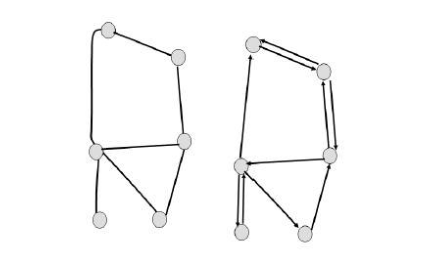
\includegraphics[width=0.50\textwidth]{./img/cap_II/5-Redes}
\caption{Exemplo do modelo de redes \cite{queirozferreira}.}
\label{fig:Redes}
\end{figure}

\subsection{Universo Estrutural}

No universo estrutural as entidades dos modelos formais são mapeadas para estruturas de dados geométricas e alfanuméricas, e algoritmos que realizam operações. As estruturas de dados utilizadas em bancos de dados geográficos podem ser divididas em duas grandes classes: estruturas vetoriais e estruturas matriciais \cite{queirozferreira}. Este trabalho se aprofundará em dados vetoriais, por não ser utilizada nenhuma estrutura matricial para representar algum tipo de dado.

As estruturas vetoriais são utilizadas para representar as coordenadas das fronteiras de cada entidade geográfica, através de três formas básicas: pontos, linhas, e áreas (ou polígonos), definidas por suas coordenadas cartesianas \cite{queirozferreira}. A Figura \ref{fig:EstruturaVetorial} ilustra as estruturas vetoriais.

\begin{figure}[h]
\centering
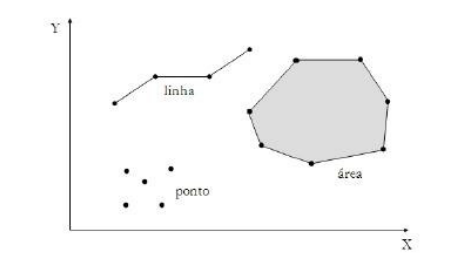
\includegraphics[width=0.55\textwidth]{./img/cap_II/6-EstruturaVetorial}
\caption{Representação das estruturas vetoriais \cite{queirozferreira}.}
\label{fig:EstruturaVetorial}
\end{figure}

\newpage

Um ponto é um par ordenado (x, y) de coordenadas espaciais. O ponto pode ser utilizado para identificar localizações ou ocorrências no espaço. Por exemplo, a localização de crimes, ocorrências de doenças, interseção de cidades. Uma linha é um conjunto de pontos conectados. A linha é utilizada para guardar feições unidimensionais. Por exemplo, um rio que conecta duas cidades distintas. Uma área (ou polígono) é a região do plano limitada por uma ou mais linhas poligonais conectadas de tal forma que o último ponto de uma linha seja idêntico ao primeiro da próxima. Os polígonos são usados para representar unidades de dados geográficos espaciais individuais como por exemplo: distritos, zonas de endereçamento postal e municípios \cite{queirozferreira}.

\subsection{Universo de Implementação}

O quarto e último paradigma contempla o universo de implementação. Neste universo são tomadas todas as decisões para codificação do sistema, como a escolha da arquitetura e a linguagem de programação a ser utilizada.

\section{Modelagem Conceitual de Dados Geográfico}

Um modelo de dados é um agrupamento de conceitos que são usados para descrever as operações e a estrutura em um banco de dados. O modelo busca sistematizar a compreensão a respeito de fenômenos e objetos que serão representados em um sistema informatizado. A modelagem de dados geográficos é bem complexa, pois envolve a discretização do espaço como parte do processo de abstração, visando obter representações adequadas aos fenômenos geográficos \cite{queirozferreira}.

Existe uma grande diferença entre esquema conceitual e modelo de dados conceitual. Esquema conceitual refere-se ao resultado de um conjunto de diagramas que usa um determinado modelo conceitual como uma linguagem para expressar estruturas de dados específicas para uma aplicação, ou seja, se refere ao resultado de uma modelagem. Já um modelo conceitual é uma técnica usada para modelar um banco de dados, incluindo sua notações \cite{queirozferreira}.

Apesar da existência de modelos para a modelagem conceitual como por exemplo, Entidade Relacionamento, \textit{Object Modeling Technique} (OTM) e \textit{Unifed Modeling Language} (UML), esses modelos não atendem as especificidades de dados espaciais. É necessário a aplicação do paradigma dos quatro universos, apresentada na seção \ref{quatro-universos}, para que seja possível agregar dados espaciais em seus modelos.

\subsection{Modelo de Dados OMT–G}
\label{modelo-omtg}

O \textit{Object Modeling Technique for Geographic Applications} (OMT-G) foi elaborado a partir das primitivas definidas do diagrama de classes da UML, adicionando-se primitivas geográficas com o objetivo de aumentar a capacidade de representação semântica do espaço. O modelo OMT-G vem com primitivas para modelar a geometria e topologia dos dados geográficos, oferecendo suporte a estruturas topológicas, estrutura de rede, múltiplas representações de objetos e relacionamentos espaciais, oferecendo também a especificação de atributos alfanuméricos e métodos ligados a cada classe \cite{omtg}.

Existe três conceitos principais para esse modelo: classes, relacionamento e restrições de integridade espaciais. Relacionamento e classes definem as primitivas básicas usadas para criação de esquemas estáticos de aplicação. Além do mais, OMT-G propõe o uso de três diferentes diagramas no processo de desenvolvimento de uma aplicação geográfica: diagrama de classes, diagrama de apresentação e diagrama de transformação, mas destes diagramas, o mais usado é o de classes, visto que ele contém as classes especificadas junto com suas representações e relacionamentos \cite{omtg}.

Por ser o diagrama mais utilizado, a seguir serão apresentadas as definições do modelo OMT-G para criação do diagrama de classes em aplicações geográficas.

\subsubsection{Classes}

Nas aplicações geográficas, encontram-se três grandes grupos de dados: os contínuos, os discretos e os não-espaciais. As classes definidas pelo modelo OMT-G representam esses três grandes grupos. Por meio delas proporcionam uma visão integrada do espaço modelado. Suas classes podem ser georreferenciadas ou convencionais. A distinção entre essas classes permite que aplicações diferentes compartilhem dados não-espaciais, facilitando o desenvolvimento de aplicações integradas e a reutilização de dados \cite{omtg}.

A classe georreferenciada descreve um conjunto de objetos que possuem representação espacial e estão associados a regiões da superfície da terra, representando as visões de geo-campos e geo-objeto (mostradas na seção \ref{quatro-universos} deste trabalho). A classe convencional descreve um conjunto de objetos com propriedades, comportamento, relacionamentos e semânticas semelhantes, e que possuem alguma relação com os objetos espaciais, mas que não possuem propriedades geográficas \cite{omtg}.

A Figura \ref{fig:ClassesOMTG} apresenta a diferença entre as classes convencionais e georreferenciadas. As classes convencionais são simbolizadas sem distinções como na UML e as classes georreferenciadas são simbolizadas no modelo OMT-G de forma semelhante, apresentando um quadrado do lado superior esquerdo designado para indicar a forma geométrica da representação. Os objetos de ambas as classes podem ou não ter atributos não espaciais associados, listados na seção central da representação completa. Operações ou métodos são especificados na seção inferior do retângulo \cite{omtg}.

\begin{figure}[h]
\centering
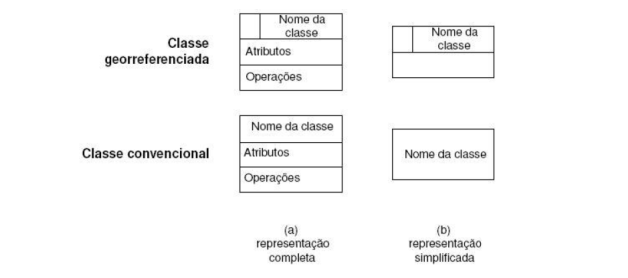
\includegraphics[width=0.70\textwidth]{./img/cap_II/7-ClassesOMTG}
\caption{Classes georreferenciadas e convencionais no OMT-G \cite{omtg}.}
\label{fig:ClassesOMTG}
\end{figure}

O modelo OMT-G apresenta um conjunto fixo de alternativas de representação geométrica, usando uma simbologia que distingue geo-campos e geo-objetos. O modelo OMT-G define cinco classes descendentes de geo-campos: (rede triangular irregular, isolinhas, subdivisão planar, tesselação e amostras) e duas descendentes de geo-objetos: (geo-objetos com geometria e geo-objetos com geometria e topologia). A Figura \ref{fig:ClassesGeo-campos} e a Figura \ref{fig:ClassesGeo-objetos} representam respectivamente as classes descendentes de geo-campos e geo-objetos \cite{omtg}.

\newpage

\begin{figure}[h]
\centering
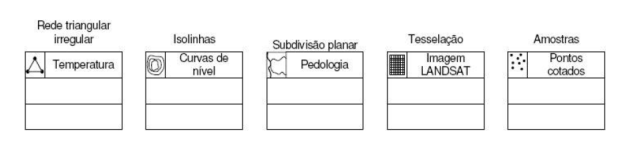
\includegraphics[width=0.70\textwidth]{./img/cap_II/8-ClassesGeo-campos}
\caption{Classes descendentes de geo-campos \cite{omtg}.}
\label{fig:ClassesGeo-campos}
\end{figure}

\begin{figure}[h]
\centering
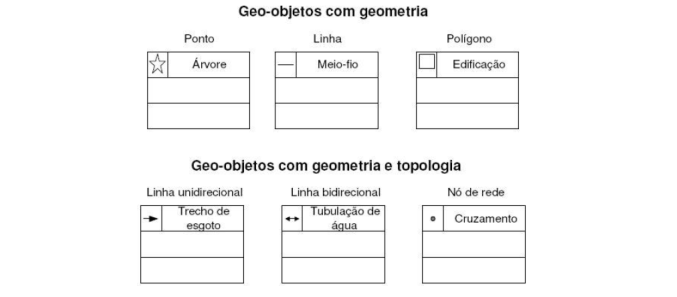
\includegraphics[width=0.70\textwidth]{./img/cap_II/9-ClassesGeo-objetos}
\caption{Classes descendentes de geo-objetos \cite{omtg}.}
\label{fig:ClassesGeo-objetos}
\end{figure}

A classe geo-objeto com geometria representa objetos que possuem apenas propriedades geométricas. Como exemplo, especializada nas classes Ponto, Linha e Polígono, indicando respectivamente, árvore, meio fio e edificação, representados nas classes de geo-objeto com geometria conforme a Figura \ref{fig:ClassesGeo-objetos} \cite{omtg}.

A classe geo-objeto com geometria e topologia representa objetos que possuem além das propriedades geométricas, propriedades de conectividade topológica, sendo especificamente voltadas para a representação de estruturas em rede, como por exemplo, sistemas de abastecimento de água ou fornecimento de energia elétrica. Essas propriedades estão presentes em classes descendentes que representam nós e arcos, da forma usualmente adotada na teoria dos grafos. Os arcos podem ser unidirecionais, como em redes de esgoto, ou bidirecionais, como em redes de telecomunicações. Na Figura \ref{fig:ClassesGeo-objetos} são representados as classes de geo-objeto com geometria e topologia \cite{omtg}.

\subsubsection{Relacionamentos}

Como as relações espaciais e não-espaciais na compreensão do espaço modelado possuem uma enorme importância, o modelo OMT-G representa três tipos de relacionamentos entre suas classes: associação simples, relacionamentos espaciais e relacionamento topológico em rede. Esses três tipos de relacionamentos têm como objetivo definir explicitamente o tipo de interação entre as classes \cite{omtg}.

Associações simples representam relacionamentos estruturais entre objetos de classes diferentes, convencionais ou georreferenciadas. No modelo OMT-G, essas associações são indicadas por linhas contínuas, como mostra a Figura \ref{fig:RelacionamentosOMTG} (a) \cite{omtg}.

Os relacionamentos espaciais representam relações topológicas e métricas. No modelo OMT-G, esse relacionamento é indicado por linhas pontilhadas como mostra a Figura \ref{fig:RelacionamentosOMTG} (b), diferentemente das associações simples, que são linhas contínuas \cite{omtg}.

\newpage

Os relacionamentos de rede são relacionamentos entre objetos que estão conectados uns com os outros. No modelo OMT-G, esses relacionamentos são representados por duas linhas pontilhadas paralelas como mostra na Figura \ref{fig:RelacionamentosOMTG} (c). Os relacionamentos são geralmente especificados entre classes de nós e uma classe de arcos. No entanto, estruturas de redes sem nós podem ser definidas, especificando um relacionamento recursivo sobre uma classe de arcos, como na Figura \ref{fig:RelacionamentosOMTG} (d) \cite{omtg}.

\begin{figure}[h]
\centering
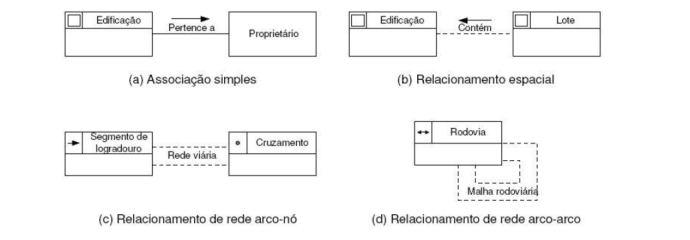
\includegraphics[width=0.80\textwidth]{./img/cap_II/10-RelacionamentosOMTG}
\caption{Relacionamentos no OMT-G \cite{omtg}.}
\label{fig:RelacionamentosOMTG}
\end{figure}

As representações de cardinalidade, generalização e especificação no modelo OMT-G seguem o mesmo padrão da diagramação UML.

\section{Sistema Gerenciador de Banco de Dados}

Um Sistema Gerenciador de Banco de Dados (SGBD) é um sistema de software que possibilita aos usuários criar e manter um banco de dados, facilitando os seguintes processos: definição, construção, manipulação e compartilhamento \cite{bancodados}.

\begin{itemize}
\item A definição de um banco de dados consiste na especificação das estruturas, dos tipos de dados e das restrições para os dados a serem armazenados no banco de dados;
\item A construção de um banco de dados é o armazenamento dos dados em alguma mídia adequada controlada pelo SGBD;
\item A manipulação ocorre a partir de um conjunto de funções, entre essas funções temos as pesquisas em banco de dados que recuperam dados especificados pelo usuário e a atualização do banco que repete as mudanças dos requisitos do banco;
\item O compartilhamento consiste no acesso concorrente ao banco de dados por múltiplos usuários e programas.
\end{itemize}

Os requisitos mais importantes para os Sistemas Gerenciadores de Banco de Dados (SGBDs) são a facilidade de uso, correção, facilidade de manutenção, confiabilidade, segurança e desempenho. Na Tabela \ref{tabela-requisitos-SGBDs} é apresentada a definição de cada requisito e a Tabela \ref{tabela-tecnologias-SGBDs} apresenta as principais tecnologias para os SGBDs a fim de cumprir esses requisitos \cite{queirozferreira}.

\newpage

\begin{table}[htbp]
\IBGEtab{
\caption{Principais requisitos para SGBDs \cite{queirozferreira, bancodados}.}
\label{tabela-requisitos-SGBDs}
}{
\begin{tabular}{ll}
\toprule
Requisito & Definição\\
\midrule \midrule
Facilidade de Uso & A modelagem do banco de dados deve refletir a realidade das aplicações e o acesso aos\\
& dados deve ser feito de forma simples\\
\midrule
Correção & Os dados armazenados no banco de dados devem refletir um estado correto\\
& da realidade modelada\\
\midrule
Facilidade de Manutenção & Alterações na forma de armazenamento dos dados devem afetar as aplicações\\
& o mínimo possível\\
\midrule
Confiabilidade & Atualizações não devem ser perdidas e não devem interferir umas com as outras\\
\midrule
Segurança & O acesso aos dados deve ser controlado de acordo com os direitos definidos para cada\\
& aplicação ou usuário\\
\midrule
Desempenho & O tempo de acesso aos dados deve ser compatível com a complexidade da consulta\\
\bottomrule
\end{tabular}}{}
\end{table}

\begin{table}[htb]
\IBGEtab{
\caption{Principais tecnologias para SGBDs \cite{queirozferreira, bancodados}.}
\label{tabela-tecnologias-SGBDs}
}{
\begin{tabular}{ll}
\toprule
Requisito & Definição\\
\midrule \midrule
Facilidade de Uso & Linguagem de definição de dados, linguagem de consulta baseada em modelo\\
& de dados de alto nível e o fornecimento de múltiplas interfaces para os usuários\\
\midrule
Correção & Restrições de integridade, \textit{triggers} e assertivas\\
\midrule
Facilidade de Manutenção & Especificações do banco de dados em níveis isolando os detalhes\\
& de armazenamento das aplicações\\
\midrule
Confiabilidade & Transações atômicas implementadas através de mecanismos para controle\\
& de concorrência, mecanismos de \textit{backup}, controle de redundância de dados e mecanismos\\
& de recuperação a caso de falhas\\
\midrule
Segurança & Níveis de autorização e controle de acesso\\
\midrule
Desempenho & Otimização de consultas, baseada em métodos de acesso e de armazenamento eficientes,\\
& gerência eficaz do \textit{buffer pool} e modelos de custo, entre outras tecnologias\\
\bottomrule
\end{tabular}}{}
\end{table}

O mercado para SGBDs concentra-se principalmente em duas tecnologias: Os SGBDs Relacionais (SGBD-R) e os SGBDs Objeto-Relacionais (SGBD-OR)\cite{queirozferreira}.

Os SGBD-R seguem o modelo relacional de dados, em que um banco de dados é organizado como uma coleção de relações, cada qual com atributos de um tipo específico. Nos sistemas comerciais atuais, os tipos incluem números inteiros, de ponto flutuante, cadeias de caracteres, datas e campos binários longos (BLOBs). Os SGBD-OR estendem o modelo relacional, entre outras características, com um sistema de tipos de dados rico e estendível, oferecendo operadores que podem ser utilizados na linguagem de consulta \cite{queirozferreira}.

Os SGBD-R foram concebidos para atender as necessidades de aplicações manipulando grandes volumes de dados convencionais. De fato, tais sistemas não oferecem recursos para atender as necessidades de aplicações não convencionais. A mera simulação de tipos de dados não convencionais em um SGBD-R pode ter efeitos colaterais, como queda de desempenho, dificuldade de codificação e posterior manutenção da aplicação. Os SGBD-OR possibilitam a extensão dos mecanismos de indexação sobre os novos tipos. Essas características reduzem os problemas ocorridos na simulação de tipos de dados pelos SGBD-R, tornando os SGBD-OR uma solução atrativa para aplicações não convencionais \cite{queirozferreira}.

Para atender as necessidades dos SIGs, surgiram SGBD-ORs com extensões geográficas \textit{open sources} como o PostGIS. No tópico seguinte, será abordado um pouco mais sobre o PostGIS.

\newpage

\section{PostGIS}

O PostGIS é uma extensão geográfica do SGBD-OR PostgreSQL desenvolvido pela empresa canadense \textit{Refractions Research}, o seu código fonte é aberto através da licença \textit{GNU PLS} \cite{PostGIS}. A Figura \ref{fig:DadosPostGIS} apresenta os tipos de dados espaciais fornecidos por essa extensão. As representações textuais desses tipos são \cite{queirozferreira}:

\begin{itemize}
\item \textit{Point: (0, 0, 0)}
\item \textit{LineString: (0 0, 1 1, 2 2)}
\item \textit{Polygon: ((0 0 0, 4 0 0, 4 4 0, 0 4 0, 0 0 0), (100, ...), ...)}
\item \textit{MultiPoint: (0 0 0, 4 4 0)}
\item \textit{MultiLineString: ((0 0 0, 1 1 0, 2 2 0), (4 4 0, 5 5 0, 6 6 0))}
\item \textit{MultiPolygon: (((0 0 0, 4 0 0 , 4 4 0, 0 4 0, 0 0 0), (...), ...), ...)}
\item \textit{GeometryCollection: (POINT(2 2 0), LINESTRING(4 4 0, 9 9 0))}
\end{itemize}

\begin{figure}[h]
\centering
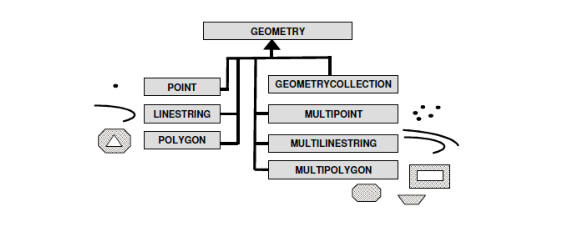
\includegraphics[width=0.70\textwidth]{./img/cap_II/11-DadosPostGIS}
\caption{Tipo de dados espaciais no PostGIS \cite{queirozferreira}.}
\label{fig:DadosPostGIS}
\end{figure}

A Figura \ref{fig:CreatePostGIS} apresenta a criação de uma tabela no PostGIS, que é realizada em duas etapas: na primeira etapa definimos os atributos básicos (alfanuméricos) e na segunda, usamos uma função para adicionar a coluna com o tipo espacial \cite{queirozferreira}.

Utilizamos a função \textit{AddGeometryColumn} para adicionar a coluna com o tipo espacial. Os parâmetros dessa função são \cite{queirozferreira}:

\begin{itemize}
\item Nome do banco de dados;
\item Nome da tabela que irá conter a coluna espacial;
\item Nome da coluna espacial;
\item Sistema de coordenadas em que se encontram as geometrias da tabela;
\item Tipo da coluna espacial, que serve para criar uma restrição que verifica o tipo do objeto sendo inserido na tabela;
\item Dimensão em que se encontram as coordenadas dos dados.
\end{itemize}

\begin{figure}[h]
\centering
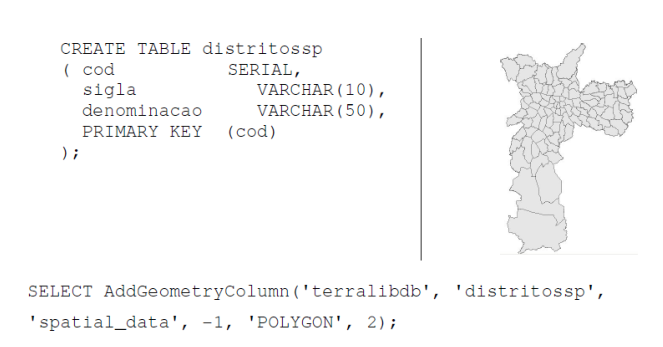
\includegraphics[width=0.70\textwidth]{./img/cap_II/12-CreatePostGIS}
\caption{Criação de uma tabela no PostGIS, adaptado de \cite{queirozferreira}.}
\label{fig:CreatePostGIS}
\end{figure}

Para inserir informações na tabela, utilizamos o comando \textit{SQL INSERT} após a criação das tabelas de dados. Para inserção da geometria, utilizamos a representação textual das geometrias em conjunto com a função \textit{GeometryFromText} que recebe a representação textual mais o sistema de coordenadas em que se encontra a geometria, apresentada na Figura \ref{fig:InsertPostGIS} \cite{queirozferreira}.

\begin{figure}[h]
\centering
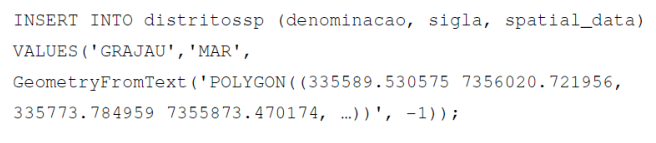
\includegraphics[width=0.70\textwidth]{./img/cap_II/13-InsertPostGIS}
\caption{Inserindo informações em uma tabela, adaptado de \cite{queirozferreira}.}
\label{fig:InsertPostGIS}
\end{figure}

A Figura \ref{fig:SelectPostGIS} apresenta um exemplo de recuperação de informações de uma tabela. O comando seleciona a linha do bairro “Vila Mariana” e utiliza a função \textit{AsText} para obter como resultado a geometria associada ao bairro de forma textual \cite{queirozferreira}.

\begin{figure}[h]
\centering
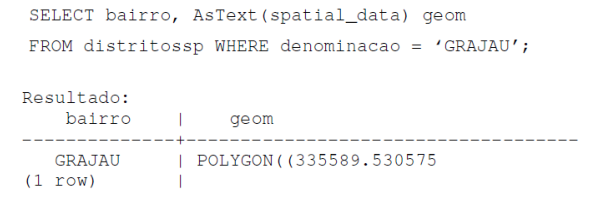
\includegraphics[width=0.70\textwidth]{./img/cap_II/14-SelectPostGIS}
\caption{Recuperando informações de uma tabela, adaptado de \cite{queirozferreira}.}
\label{fig:SelectPostGIS}
\end{figure}

\newpage

Na Figura \ref{fig:IndexPostGIS}, é apresentada a sintaxe básica para a criação de uma indexação espacial e um exemplo de criação em uma tabela \cite{queirozferreira}.

\begin{figure}[h]
\centering
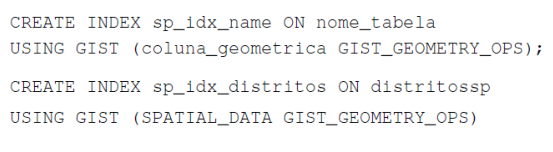
\includegraphics[width=0.70\textwidth]{./img/cap_II/15-IndexPostGIS}
\caption{Indexação espacial, adaptado de \cite{queirozferreira}.}
\label{fig:IndexPostGIS}
\end{figure}

Os índices espaciais são usados em consultas que envolvem predicados espaciais, como no caso de consultas por janela, no qual um retângulo é informado e as geometrias que interagem com ele devem ser recuperadas rapidamente.

\section{Consultas Espaciais}

O PostGIS possui vários operadores espaciais disponíveis que são fornecidos através da integração do PostGIS com a biblioteca \textit{Geometry Engine Open Source} (GEOS). A Figura \ref{fig:OperadoresPostGIS} mostra uma relação de vários operadores disponíveis \cite{queirozferreira}.

\begin{figure}[h]
\centering
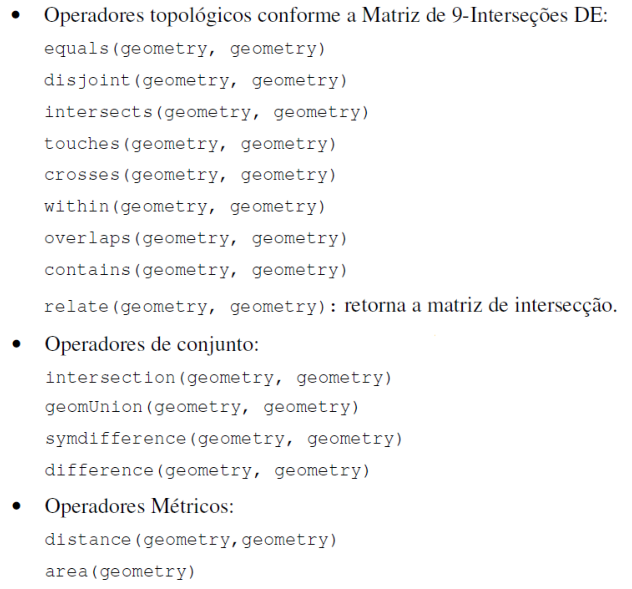
\includegraphics[width=0.70\textwidth]{./img/cap_II/16-OperadoresPostGIS}
\caption{Operadores espaciais disponíveis no PostGIS, adaptado de \cite{queirozferreira}.}
\label{fig:OperadoresPostGIS}
\end{figure}

\newpage

Em \citeonline{spatialjoins}, as consultas espaciais são classificadas nos seguintes itens:

\begin{itemize}
\item Seleção espacial: determina todos os objetos de um conjunto de objetos espaciais cujas geometrias satisfazem um predicado de seleção espacial;
\item Junção espacial: determina todos os pares de dois conjuntos de objetos espaciais cujas geometrias satisfazem um predicado de seleção espacial.
\end{itemize}

São identificados casos particulares importantes na seleção espacial \cite{spatialjoins}:

\begin{itemize}
\item Seleção por ponto: determina todos os objetos de um conjunto de objetos espaciais cujas geometrias contêm um ponto dado;
\item Seleção por região: determina todos os objetos de um conjunto de objetos espaciais cujas geometrias estão contidas em uma região dada;
\item Seleção por janela: determina todos os objetos de um conjunto de objetos espaciais cujas geometrias estão contidas em um retângulo com os lados paralelos aos eixos dados.
\end{itemize}

A Figura \ref{fig:SelecaoEspacial} apresenta o resultado de uma seleção espacial. Na Figura é selecionado as regiões da França adjacentes à região de \textit{Midi-Pirenées} (a região de \textit{Midi-Pirenées} aparece em cinza escuro e as regiões adjacente em cinza claro).

\begin{figure}[h]
\centering
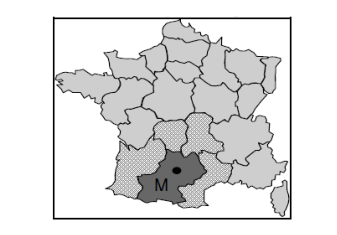
\includegraphics[width=0.50\textwidth]{./img/cap_II/17-SelecaoEspacial}
\caption{Operação de seleção espacial \cite{queirozferreira}.}
\label{fig:SelecaoEspacial}
\end{figure}

A Figura \ref{fig:JuncaoEspacial} apresenta o resultado de um junção espacial. Na consulta é utilizado o operador  espacial \textit{SDO\_TOUCH} que retorna verdadeiro caso as geometrias de d2 toquem a geometria de Grajaú. Esse é um exemplo de junção espacial entre duas relações (no nosso caso a mesma relação foi empregada duas vezes), utilizando o índice espacial \cite{queirozferreira}.

\newpage

\begin{figure}[h]
\centering
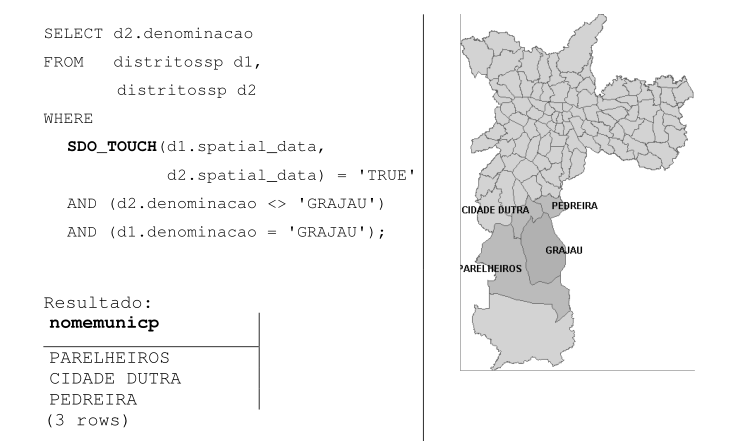
\includegraphics[width=0.75\textwidth]{./img/cap_II/19-JuncaoEspacial}
\caption{Operação de junção espacial \cite{queirozferreira}.}
\label{fig:JuncaoEspacial}
\end{figure}